\documentclass[12pt,compress,aspectratio=169]{beamer}
\usetheme{metropolis}
\setbeamersize{text margin left=.5cm,text margin right=.5cm}
\usepackage[lf]{carlito}
\usepackage{siunitx}
\usepackage{tikz}
\usepackage{mathpazo}
\usepackage{bm}
\usepackage{mathtools}
\usepackage[ISO]{diffcoeff}
\diffdef{}{ op-symbol=\mathsf{d} }
\usepackage{xcolor,colortbl}


\usetikzlibrary{decorations.pathmorphing,patterns}


\title{Topic 3: Work and Energy}
\subtitle{Advanced Placement Physics C}
\author[TML]{Dr.\ Timothy Leung}
\institute{Olympiads School}
\date{Updated: Summer 2022}

\newcommand{\pic}[2]{
  \includegraphics[width=#1\textwidth]{#2}
}
\newcommand{\eq}[2]{
  \vspace{#1}{\Large
    \begin{displaymath}
      #2
    \end{displaymath}
  }
}
%\newcommand{\iii}{\ensuremath\hat{\bm{\imath}}}
%\newcommand{\jjj}{\ensuremath\hat{\bm{\jmath}}}
%\newcommand{\kkk}{\ensuremath\hat{\bm{k}}}
%\newcommand{\iii}{\ensuremath\hat x}
%\newcommand{\jjj}{\ensuremath\hat y}
%\newcommand{\kkk}{\ensuremath\hat z}



\begin{document}

\begin{frame}
  \maketitle
\end{frame}



\begin{frame}{Work and Energy}
  We start with some definition at are (unfortunately) not very useful:
  \begin{itemize}
    \item \textbf{Energy} is the ability to do work.
    \item \textbf{Work} is the mechanism in which energy is transformed.
  \end{itemize}
  Luckily, we can also use equations to define these concepts.
\end{frame}


\section{Work}

\begin{frame}{Work}
  \textbf{Mechanical work} $\dl W$ is performed when a force $\bm F$ displaces
  an object by $\dl\bm x$. If a varying force is applied to move an object from
  $\bm x_1$ to $\bm x_2$ along a path, then the total work done by the force is
  defined by the integral:

  \eq{-.2in}{
    W=\int_{x_1}^{x_2}\bm F(\bm x)\cdot\dl\bm x
  }

  \begin{itemize}
  \item Work is a scalar quantity
  \item No work done if the force is perpendicular to displacement, when
    $\bm F\cdot\dl\bm x=0$ (i.e.\ the force did not cause the displacement)
  \item No work done if no displacement ($\dl\bm x=\bm 0$)
  \item Work can be positive or negative depending on the dot product
  \item When there are multiple forces acting on an object, we can compute the
    work done by each \emph{each} force
  \end{itemize}
\end{frame}



\begin{frame}{Work by Constant Force}
  For a constant force, if the object moves along straight path, the integral
  simplifies to just the dot product of the two vectors:

  \eq{-.2in}{
    \boxed{
      W=\bm F\cdot\Delta\bm x
    }
  }

  Or in the scalar form that is more familiar in Grades 11/12 Physics that
  avoid vector notations:

  \eq{-.2in}{
    \boxed{W=F\Delta x\cos\theta}
  }

  \vspace{-.1in}where $\theta$ is the angle between the force and displacement
  vectors
\end{frame}



\begin{frame}{Definition of Work}
  \textbf{Work done by a force}
  \begin{itemize}
  \item The work done by \emph{one specific force}
  \item Example: A boy pushes a cart forward. The ``work done by the boy'' is
    the work done by the applied force.
  \end{itemize}

  \vspace{.15in}\textbf{Work done on an object}
  \begin{itemize}
  \item There may be more than one force acting on an object
  \item The \emph{sum} of all the work done on the object by each force
  \item The work done by the net force
  \item Also called the \textbf{net work} $W_\text{net}$
  \end{itemize}
\end{frame}



\section{Kinetic Energy \& Work-Energy Theorem}

\begin{frame}{Kinetic Energy}
  When a net force on an object (with constant mass) accelerates it, the
  resulting amount of work done on the object (net work $W_\text{net}$) is
  given by:

  \eq{-.3in}{
    W_\text{net}
    =\int_{x_1}^{x_2}\bm F_\text{net}\cdot\dl\bm x
    =\int_{x_1}^{x_2}m\bm a\cdot\dl\bm x
    =m\int_{x_1}^{x_2}\diff{\bm v}t\cdot\dl\bm x
  }

  Both $\bm v$ and $\bm x$ are continuous functions in time, we can switch
  the order of differentiation. %Also, since $\bm v$ and $d\bm v$ must be in
  %the same direction, the dot product is trivial: $\bm v\cdot d\bm v=vdv$

  \eq{-.2in}{
    =m\int\diff{\bm x}t\cdot\dl\bm v=m\int\bm v\cdot\dl\bm v
    =m\int_{v_1}^{v_2}v\dl v
  }
\end{frame}



\begin{frame}{Kinetic Energy}
  This integral, when integrated from $v_1$ (initial \emph{speed}) to $v_2$
  (final \emph{speed}), becomes:

  \eq{-.2in}{
    =m\int_{v_1}^{v_2}v\dl v
    =\frac12mv^2\Big|^{v_2}_{v_1}
    =\frac12mv_2^2-\frac12mv_1^2
    =\Delta K
  }
  
  where $K$ is defined as the \textbf{translational kinetic energy}:

  \eq{-.1in}{
    \boxed{
      K=\frac12mv^2
    }
  }

  Later in the course we will discuss \emph{rotational} kinetic energy.
\end{frame}



\begin{frame}{Work and Kinetic Energy}
  In fact, the \emph{definition} of kinetic energy came from this integration,
  in that work equals to the change in \emph{something}, and we define that as
  kinetic energy. This is the \textbf{work-energy theorem}:

  \eq{-.15in}{
    \boxed{
      W_\text{net}=\Delta K
    }
  }
  \begin{itemize}
  \item\vspace{-.15in} $\Delta K$ can be positive or negative depending on the
    dot product
  \item When multiple forces acting on an object; each force can add or remove
    kinetic energy from an object
  \item Therefore we use the ``net'' amount of work done in the above equation
  \end{itemize}
\end{frame}



\begin{frame}{Example}
  \textbf{Example 1:} A force $\bm F=4.0x\bm{\hat{\imath}}$ (in newtons) acts
  on an object of mass \SI{2.}{\kilo\gram} as it moves from $x=1.0$ to
  $x=\SI{5.}\metre$. Given that the object is at rest at $x=1$,
  \begin{enumerate}[(a)]
  \item Calculate the net work
  \item What is the final speed of the object?
  \end{enumerate}
\end{frame}



\section{Potential Energy}

\begin{frame}{Gravitational Force \& Gravitational Potential Energy}
  Consier an object that is free-falling under the force of gravity over a
  distance of $\Delta x$:

  \begin{center}
    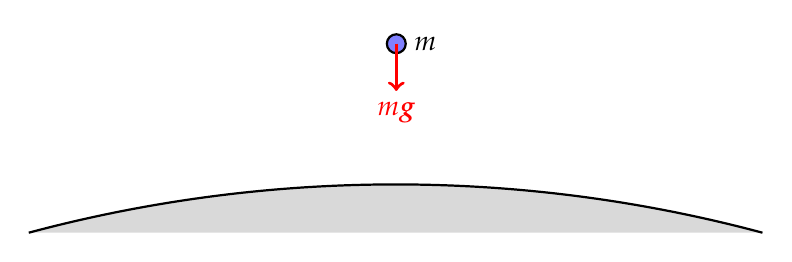
\begin{tikzpicture}[scale=.6]
      \draw[thick,fill=gray!30] (7.75,0) arc(75:105:30);
      \draw[thick,fill=blue!50] (0,4) circle(.2) node[right]{$\;m$};
`      \draw[very thick, red,->] (0,4)--(0,3) node[below]{$m\bm g$};
    \end{tikzpicture}
  \end{center}
  \begin{itemize}
  \item Assuming that $\Delta\bm x$ is small, $\bm g$ can be considered to be
    constant
  \item The work done by the gravity ($W_g$) is \emph{positive}, and
    therefore, there is an increase in kinetic energy. The object speeds up.

    \eq{-.2in}{
      W_g=mg\Delta x=\Delta K > 0
    }
  \end{itemize}
\end{frame}



\begin{frame}{Gravitational Potential Energy}
  The work done by gravity can also be expressed in terms of the change in
  height. Using ground as the reference level (i.e.\ $h=0$):
  \begin{center}
    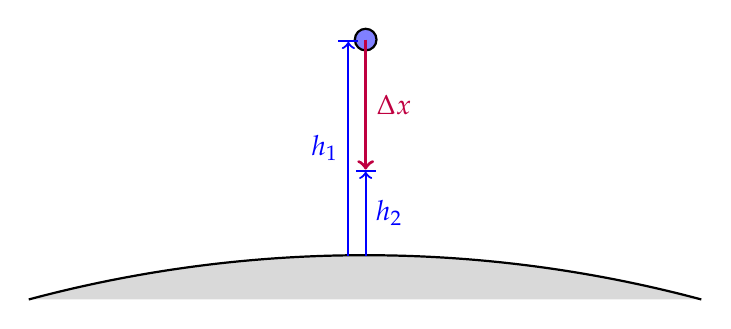
\begin{tikzpicture}[scale=.55]
      \draw[thick,fill=gray!30] (7.75,0) arc(75:105:30);
      \draw[thick,fill=blue!50] (0,6) circle(.25);
      \draw[very thick,purple,->](0,6)--(0,3) node[midway,right]{$\Delta x$};
      \draw[thick,->|,blue](-.4,1)--(-.4,6) node[midway,left]{$h_1$};
      \draw[thick,->|,blue](0,1)--(0,3) node[midway,right]{$h_2$};
    \end{tikzpicture}
  \end{center} 
%  
%  \eq{-.25in}{
%    \bm{w}=m\bm{g}
%  }
%  
%  \vspace{-.1in}Near Earth's surface, we assume that
%  $\bm{g}$ %=-g\bm{\hat{\jmath}}\approx -10\bm{\hat{\jmath}}$
%  %\si{\metre\per\second\squared}
%  is constant. The work done to move an object from height $h_1$ to $h_2$ is
%  therefore:

  \vspace{-.3in}{\Large
    \begin{align*}
      W_g
      &= mg(h_2-h_1)\\
      &= -mg(h_2-h_1)=-(mgh_2-mgh_1)
    \end{align*}
  }


\end{frame}



\begin{frame}{Gravitational Potential Energy}
  Defining the \textbf{gravitational potential energy} $U_g$ as:

  \eq{-.2in}{
    \boxed{U_g=mgh}
  }

  The the work done by gravity can be related to this potential energy by:
  
  \eq{-.2in}{
    \boxed{  W_g=-\Delta U_g }
  }

  \fbox{
    \begin{minipage}{.95\textwidth}
      \begin{itemize}
      \item \emph{Positive} work decreases gravitational potential energy, while
      \item \emph{Negative} work increases gravitational potential energy
      \item $W_g$ depends on the end points $h_1$ and $h_2$, but not \emph{how}
        it went from $h_1\rightarrow h_2$
      \end{itemize}
    \end{minipage}
  }
\end{frame}




\begin{frame}{Spring Force \& Elastic Potential Energy}
  The spring force $\bm F_s$ is the force that a compressed/stretched spring
  exerts on the object connected to it. An \emph{ideal} spring obeys Hooke's
  law:
  
  \eq{-.2in}{
    \bm F_s=-k\bm x
  }

  \vspace{-.15in}The work done by the spring force as it pushes any masses that
  are connected to a compressed/stretched spring is therefore:

  \vspace{-.3in}{\Large
    \begin{align*}
      W=\int_{x_1}^{x_2}\bm F_s\cdot\dl\bm x &=-k\int_{x_1}^{x_2} x\dl x\\
      &=-\frac12kx^2\Big|^{x_2}_{x_1}=-\left[\frac12kx_2^2-\frac12kx_1^2\right]
    \end{align*}
  }
\end{frame}



\begin{frame}{Elastic Potential Energy}
  Defining the \textbf{elastic potential energy} $U_e$ as:

  \eq{-.2in}{
    \boxed{
      U_e=\frac12kx^2
    }
  }

  The the work done by the spring force can be related to the elastic
  potential energy by:
  
  \eq{-.2in}{
    \boxed{  W_s=-\Delta U_e }
  }

  \fbox{
    \begin{minipage}{.95\textwidth}
      \begin{itemize}
      \item \emph{Positive} work by the spring decreases spring potential
        energy, while
      \item \emph{Negative} work by the spring increases spring potential energy
      \item $W_s$ depends on the end points $x_1$ and $x_2$, but not \emph{how}
        it went from $x_1\rightarrow x_2$
      \end{itemize}
    \end{minipage}
  }
\end{frame}



\begin{frame}{Conservative Forces}
  Gravitational force $\bm F_g$, spring force $\bm F_s$, electrostatic force
  $\bm F_q$ (studied in Physics 12, and later in the course), magnetic force
  $\bm F_m$, and nuclear forces are \textbf{conservative forces}
  \begin{itemize}
  \item The work done by these forces relate to a change of a related
    potential energy
    \begin{itemize}
    \item Positive work decreases this related potential energy,
    \item Negative work increases this related potential energy
    \end{itemize}
  \item The work done by a conservative force is \emph{path independent}
    (depends only on end points)
  \end{itemize}
\end{frame}



\begin{frame}{Conservative Forces}
  By the fundamental theorem of calculus, any conservative forces $\bm F$
  must be the negative gradient of the potential energies:

  \eq{-.2in}{
    \bm F=-\nabla U=
    -\diffp Ux\bm{\hat{\imath}}-\diffp Uy\bm{\hat{\jmath}}-\diffp Uz\hat{\bm{k}}
  }

  In one-dimension:

  \eq{-.2in}{
    \boxed{
      F=-\diff Ux
    }
  }

  The direction of a conservative force \emph{always} decreases the potential
  energy. (Pay attention to the negative sign. Students often forget it.)
\end{frame}




%\begin{frame}{Work and Potential Energy}
%  The expressions for potential energies also come from integrating the work
%  equation, in that work equals to the change in \emph{something}, and we
%  called that potential energy. Therefore:
%
%  \eq{-.2in}{
%    \boxed{
%      W_c=-\Delta U
%    }
%  }
%  \begin{itemize}
%  \item\vspace{-.15in}$\Delta U$ can be positive or negative depending on the
%    direction of the (conservative) force
%  \item Positive work \emph{decreases} the related potential energy
%  \item Negative work \emph{increases} the related potential energy
%  \end{itemize}
%\end{frame}



\begin{frame}{Conservation of Mechanical Energy}
  Positive work done by conservative forces on an object does two things:
  \begin{enumerate}[1.]
  \item Decrease its potential energy, while
  \item Increase its kinetic energy by the same amount
  \end{enumerate}
  Mathematically, this shows that mechanical energy must \emph{always} be
  conserved when there are only conservative forces:

  \eq{-.15in}{
    W_c=-\Delta U = \Delta K \quad\longrightarrow\quad
    \Delta K + \Delta U =0
  }

  That's why those forces are called conservative forces!
\end{frame}


\section{Non-Conservative Forces}

\begin{frame}{Examples of Non-Conservative Force}
  The majority of forces are \textbf{non-conservative}. Here are some examples:
  \begin{itemize}
  \item Work done by these forces are \emph{usually} negative because they
    oppose the direction of motion
    \begin{itemize}
    \item Drag (fluid resistance)
    \item Friction\footnote{but sometimes it can also do positive work too.}
    \end{itemize}
  \item The work done by these forces may be positive or negative, depending on
    the problem
    \begin{itemize}
    \item Applied force
    \item Tension force
    \item Normal force
    \end{itemize}
  \end{itemize}
  \textbf{The work-energy theorem still applies for non-conservative forces}
\end{frame}



\begin{frame}{Work by Non-Conservative Forces}
  The work done by non-conservative forces differs from conservative forces in
  that:
  \begin{itemize}
  \item There is no related potential energies: the work done by a
    non-conservative force transform energy from one form of kinetic energy to
    another
  \item The work is path dependent
  \end{itemize}
\end{frame}



\begin{frame}{Work by Friction, an Illustration}
  Work by frictional force---and other non-conservative forces---is illustrated
  below. Two blocks ($m_1$ and $m_2$), stacked vertically, move to the right by
  external force.% $\bm F$ applied to $m_1$.
  \begin{center}
    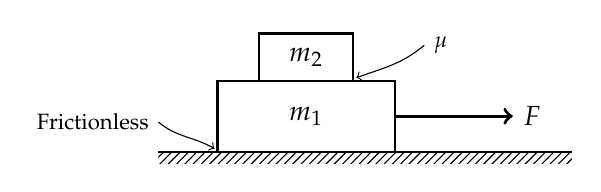
\begin{tikzpicture}[scale=.75]
      \fill[pattern=north east lines](0,0) rectangle(7,-.2);
      \draw[thick](0,0)--(7,0);
      \draw[thick](1,0)     rectangle(4,1.2) node[midway]{$m_1$};
      \draw[thick](1.7,1.2) rectangle(3.3,2) node[midway]{$m_2$};
      \draw[->,very thick](4,.6)--(6,.6)     node[right] {$F$};
      \draw[<-](0.95,0.05)to[out=150,in=-40](0,.5)
      node[left]{\footnotesize Frictionless};
      \draw[<-](3.35,1.25)to[out=20, in=220](4.5,1.8)
      node[right]{\footnotesize $\mu$};
    \end{tikzpicture}
  \end{center}
  The FBDs of the blocks are shown below. (The forces highlighted in the same
  color are action-reaction pairs.)
  \begin{center}
    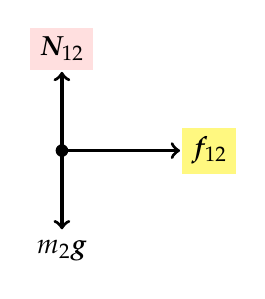
\begin{tikzpicture}
      \fill(0,0) circle(.08);
      \begin{scope}[->,very thick]
        \draw(0,0)--(0,-1) node[below]{$m_2\bm g$};
        \draw(0,0)--(0, 1) node[above,fill=pink!50]{$\bm N_{12}$};
        \draw(0,0)--(1.5,0)node[right,fill=yellow!50]{$\bm f_{12}$};
      \end{scope}
    \end{tikzpicture}
    \hspace{.2in}
    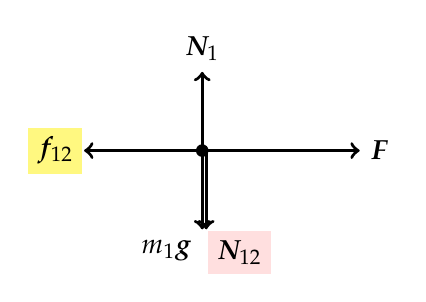
\begin{tikzpicture}
      \fill(0,0) circle(.08);
      \begin{scope}[->,very thick]
        \draw(0,0)--(0,-1) node[below left]{$m_1\bm g$};
        \draw(.05,0)--(.05,-1) node[below right,fill=pink!50]{$\bm N_{12}$};
        \draw(0,0)--(0, 1) node[above]{$\bm N_1$};
        \draw(0,0)--(-1.5,0)node[left,fill=yellow!50]{$\bm f_{12}$};
        \draw(0,0)--(2,0)node[right]{$\bm F$};
      \end{scope}
    \end{tikzpicture}
  \end{center}
\end{frame}



\begin{frame}{Work Done By Friction}
  \begin{columns}
    \column{.25\textwidth}
    \centering
    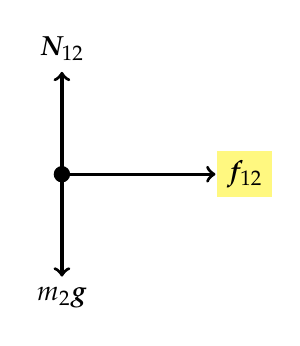
\begin{tikzpicture}[scale=1.3]
      \fill(0,0) circle(.08);
      \begin{scope}[->,very thick]
        \draw(0,0)--(0,-1) node[below]{$m_2\bm g$};
        \draw(0,0)--(0, 1) node[above]{$\bm N_{12}$};
        \draw(0,0)--(1.5,0)node[right,fill=yellow!50]{$\bm f_{12}$};
      \end{scope}
    \end{tikzpicture}

    \column{.75\textwidth}
    For the top block $m_2$, when it moves to the right
    \begin{itemize}
    \item Friction between the blocks $\bm f_{12}$ is the only force doing work
    \item The work done by $\bm f_{12}$ is positive
    \item Mass $m_2$ gains kinetic energy
    \end{itemize}
  \end{columns}
  \begin{columns}
    \column{.6\textwidth}
    For the bottom block $m_1$, when it moves to the right
    \begin{itemize}
    \item Applied force $\bm F$ does positive work on $m_1$, while
    \item Friction between the blocks $\bm f_{12}$ does negative work
    \item Therefore $\bm f_{12}$ decreases the kinetic energy
    \end{itemize}
    
    \column{.4\textwidth}
    \centering
    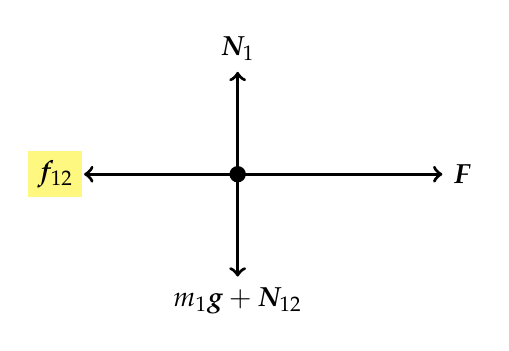
\begin{tikzpicture}[scale=1.3]
      \fill(0,0) circle(.08);
      \begin{scope}[->,very thick]
        \draw(0,0)--(0,-1) node[below]{$m_1\bm g+\bm N_{12}$};
        \draw(0,0)--(0, 1) node[above]{$\bm N_1$};
        \draw(0,0)--(-1.5,0)node[left,fill=yellow!50]{$\bm f_{12}$};
        \draw(0,0)--(2,0)node[right]{$\bm F$};
      \end{scope}
    \end{tikzpicture}    
  \end{columns}
\end{frame}



\begin{frame}{Work by Friction}
  The work done by friction is
  \begin{itemize}
  \item positive on one object
  \item negative on another
  \end{itemize}
  Therefore, work by non-conservative forces transforms energy from the kinetic
  energy of one object into the kinetic energy of another object.
\end{frame}



\section{Conservation of Energy}

\begin{frame}{Isolated Systems and the Conservation of Energy}
  An \textbf{isolated system} is a system of objects that does not interact with
  the surrounding. Think of an isolated system as a bunch of objects inside an
  insulated box.
  \begin{center}
    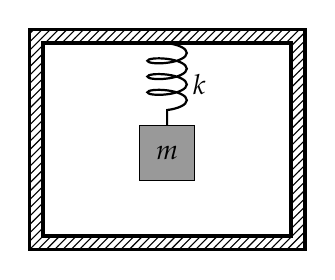
\begin{tikzpicture}[scale=.7]
      \fill[pattern=north east lines] (0,0) rectangle(5,4);
      \draw[very thick] (0,0) rectangle(5,4);
      \draw[very thick,fill=white](.25,.25) rectangle(4.75,3.75);
      \draw[thick,
        decoration={aspect=.3,segment length=2mm, amplitude=2.5mm, coil},
        decorate] (2.5,3.75)--(2.5,2.25) node[midway,right]{$\;\;k$};
      \draw[fill=black!40](2,2.25) rectangle(3,1.25) node[midway]{$m$};
    \end{tikzpicture}
  \end{center}
  Since the system is isolated from the surrounding environment, the
  environment can't do any work on it. Likewise, the energy inside the system
  cannot escape either.
\end{frame}



\begin{frame}{Example: Horizontal Spring-Mass System}
  Assuming that there are no friction, drag or other damping forces present, a
  horizontal spring-mass system is a closed system:
  \begin{center}
    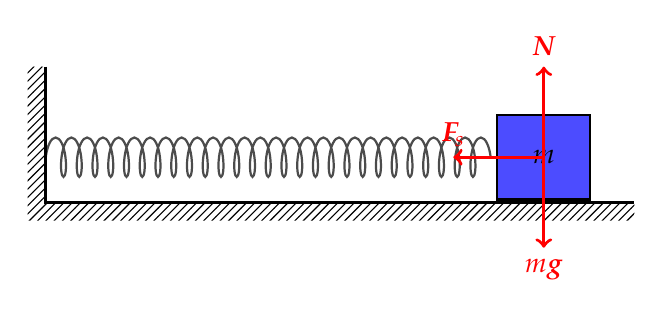
\begin{tikzpicture}[scale=1.15]
      \node[draw=black,thick,fill=blue!70,inner sep=4.5mm] (a) at (5.5,1) {$m$};
      \draw[thick,draw=black!70,
        decoration={aspect=.3,segment length=2mm, amplitude=2.5mm, coil},
        decorate] (0,1)--(4.95,1);
      \fill [pattern=north east lines] (6.5,.5)--(6.5,.3)--(-.2,.3)
      --(-.2,2)--(0,2)--(0,.5)--cycle;
      \draw[very thick] (0,2)--(0,.5)--(6.5,.5);
      \begin{scope}[very thick,->,red]
        \draw (5.5,1)--(5.5,0) node[below]{$m\bm g$};
        \draw (5.5,1)--(5.5,2) node[above]{$\bm N$};
        \draw (5.5,1)--(4.5,1) node[above]{$\bm F_s$};
      \end{scope}
    \end{tikzpicture}
  \end{center}
  \begin{itemize}
  \item The only force doing work is the spring force (conservative!) on the
    mass.
  \item The sum of the kinetic energy of the mass ($K$) and the elastic
    potential energy stored in the spring ($U_e$) is constant

    \eq{-.25in}{
      K+U_e=\text{constant}
    }
  \end{itemize}
\end{frame}



\begin{frame}{Example: Gravity}
  Assuming that there is no friction and drag, a free-falling object forms a
  closed system with Earth:
  \begin{center}
    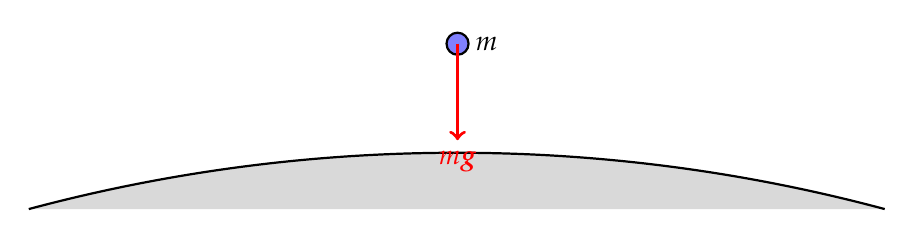
\begin{tikzpicture}[scale=.7]
      \draw[thick,fill=gray!30] (7.75,0) arc(75:105:30);
      \draw[thick,fill=blue!50] (0,3) circle(.2) node[right]{$\;m$};
      \draw[very thick, red,->] (0,3)--(0,1.25) node[below]{$m\bm g$};
    \end{tikzpicture}
  \end{center}
  \begin{itemize}
  \item The only force doing work is gravity (conservative!) on the mass
  \item The sum of the kinetic energy of the mass ($K$) and the gravitational
    potential energy stored between the tow masses ($U_g$) is constant
    
    \eq{-.1in}{
      K+U_g=\text{constant}
    }
  \end{itemize}
\end{frame}



\begin{frame}{Example: Vertical Spring-Mass System}
  \begin{columns}
    \column{.25\textwidth}
    \centering
    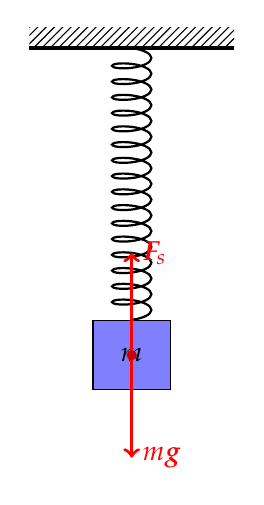
\begin{tikzpicture}[scale=1.3]
      \node[draw=black,fill=blue!50,inner sep=3.5mm] (b) at (1,2) {$m$};
      \draw[thick,
        decoration={aspect=.3,segment length=2mm, amplitude=2.5mm, coil},
        decorate] (1,5)--(b); 
      \fill [pattern=north east lines] (0,5) rectangle (2,5.2);
      \draw[very thick] (0,5)--(2,5);
      \begin{scope}[very thick,->,red]
        \draw(1,2)--(1,1)node[right]{$m\bm g$};
        \draw(1,2)--(1,3)node[right]{$\bm F_s$};
      \end{scope}
      \fill[red!80!black](1,2) circle(.05);

      
    \end{tikzpicture}

    \column{.75\textwidth}
    Assuming that there are no friction, drag or other damping forces in the
    spring, the vertical spring-mass system (consists of the mass, the spring
    and Earth) is a closed system.
    \begin{itemize}
    \item Both gravity and spring force are doing work
    \item The sum of the kinetic energy of the mass ($K$), the gravitational
      potential energy stored between the mass and Earth ($U_g$), and the
      elastic potential energy stored in the spring ($U_e$) is constant.

      \eq{-.1in}{
          K + U_g + U_e=\text{constant}
      }
    \end{itemize}
  \end{columns}
\end{frame}



\begin{frame}{Simple Pendulum System}
  \begin{columns}
    \column{.7\textwidth}
    Assuming that there are no friction, drag or other damping forces in the
    spring, the simple pendulum system (consists of the mass and Earth) is a
    closed system.
    \begin{itemize}
    \item Gravity ($m\bm g$), which is conservative, is the only force that
      does work
    \item Tension ($\bm T$) does not do work on the pendulum because it is
      perpendicular to the motion of the pendulum bob
    \item The sum of the kinetic energy of the mass ($K$), the gravitational
      potential energy stored between the mass and Earth ($U_g$) is constant:

      \eq{-.1in}{
          K + U_g =\text{constant}
      }
    \end{itemize}
    
    \column{.3\textwidth}
    \centering
    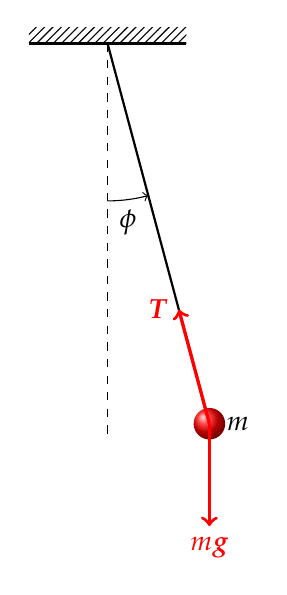
\begin{tikzpicture}
      \fill[pattern=north east lines] (-1,0) rectangle (1,0.2);
      \draw[thick](-1,0)--(1,0);
      \begin{scope}[rotate=15]
        \draw[thick](0,0)--(0,-5);
        \tikzstyle{balloon}=[ball color=red];    
        \shade[balloon] (0,-5) circle(.2) node[right]{$\;m$};
        \begin{scope}[red,very thick,->]
          \draw(0,-5)--(0,-3.5) node[left]{$\bm T$};
          \draw[rotate around={-15:(0,-5)}](0,-5)--(0,-6.3)
          node[below]{$m\bm g$};
        \end{scope}
      \end{scope}
      \draw[dashed,thin](0,0)--(0,-5);
      \draw[->](0,-2) arc(270:285:2) node[midway,below]{$\phi$};
    \end{tikzpicture}
  \end{columns}
\end{frame}


\begin{frame}{What if there is friction?}
  Energy is always conserved as long as your system is defined properly. In
  this case, the system consists of a mass, a spring, Earth and all the air
  molecules inside the box:
  \begin{center}
    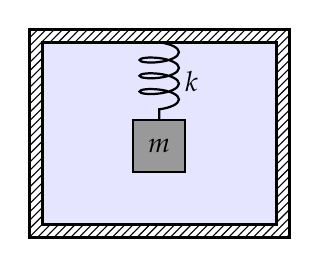
\begin{tikzpicture}[scale=.66]
      \fill[pattern=north east lines] (0,0) rectangle(5,4);
      \draw[very thick] (0,0) rectangle(5,4);
      \draw[very thick,fill=blue!10](.25,.25) rectangle(4.75,3.75);
      \draw[thick,
        decoration={aspect=.3,segment length=2mm, amplitude=2.5mm, coil},
        decorate] (2.5,3.75)--(2.5,2.25) node[midway,right]{$\;\;k$};
      \draw[thick,fill=black!40](2,2.25) rectangle(3,1.25) node[midway]{$m$};
    \end{tikzpicture}
  \end{center}
  The energies of this system include
  \begin{itemize}
  \item Kinetic energy of the mass ($K$)
  \item Gravitational potential energy ($U_g$) between the mass and Earth
  \item Elastic potential energy ($U_e$) stored in the spring
  \item Thermal (kinetic) energy ($K_\text{air}$) of the vibration of the air
    molecules
  \end{itemize}
\end{frame}



\begin{frame}{Conservation of Energy with Non-Conservative Forces}
  As the mass vibrates, friction and drag with air slows it down, while the
  temperature of the air rises due to friction and drag. Total energy is
  conserved even as the mass stops moving

  \vspace{.2in}
  \begin{columns}
    \column{.4\textwidth}
    \centering
    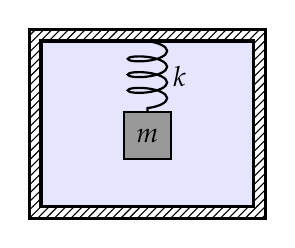
\begin{tikzpicture}[scale=.6]
      \fill[pattern=north east lines] (0,0) rectangle(5,4);
      \draw[very thick] (0,0) rectangle(5,4);
      \draw[very thick,fill=blue!10](.25,.25) rectangle(4.75,3.75);
      \draw[thick,
        decoration={aspect=.3,segment length=2mm, amplitude=2.5mm, coil},
        decorate] (2.5,3.75)--(2.5,2.25) node[midway,right]{$\;\;k$};
      \draw[thick,fill=black!40](2,2.25) rectangle(3,1.25) node[midway]{$m$};
    \end{tikzpicture}

    \column{.6\textwidth}
    \eq{0pt}{
      K + K_\text{air}+U_g+U_e=\text{constant}
    }
  \end{columns}

  \vspace{.2in}Non-conservative forces doing work are \emph{internal} to the
  system, and therefore energy is still conserved. (Work done by friction
  transform from the kinetic energy of the mass to the kinetic energy of the
  air molecules.)
\end{frame}



\begin{frame}{Conservation of Energy}
  If \emph{only} conservative forces are doing work, mechanical energy (i.e.\
  $K+U$) is always conserved:

  \eq{-.2in}{
    \boxed{K +U =K'+U'}
  }
  
  When external non-conservative forces are also doing work, instead of
  \emph{trying} to isolate the system, we can instead calculate the work done
  by them $W_{nc}$ and add it to the total energy of the system
    
  \eq{-.2in}{
    \boxed{K+U+W_{nc}=K'+U'}
  }
\end{frame}



\begin{frame}{Example}
  \textbf{Example 2:} A mass $m$ is dropped from a height of $h$ above the
  equilibrium position of a spring. Set up the equation that determines the
  spring's compression $d$ when the object is instantaneously at rest.
  \begin{center}
    \pic{.35}{spring-example1}
  \end{center}
\end{frame}


%\begin{frame}{Example}
%  \textbf{Example 3:} A mass $m$ is pulled a distance $d$ up an incline (angle
%  of elevation $\theta$) at constant speed using a rope that is parallel to
%  the incline. The coefficient of friction is $\mu_k$.
%  \begin{enumerate}[(a)]
%  \item What is the magnitude of the tension force in the rope?
%  \item What is the magnitude of the normal force?
%  \item What is the work done by the normal force?
%  \item What is the work done by friction?
%  \item What is the work done by the tension force?
%  \item What is the net work?
%  \item What is the change in total mechanical energy?
%  \item Show that $\Delta E_{mech}=W_{nc}$.
%  \end{enumerate}
%\end{frame}


\begin{frame}{Energy Diagrams}
  Plot of potential energy ($U$) vs.\ position ($x$) for a conservative force
  \begin{center}
    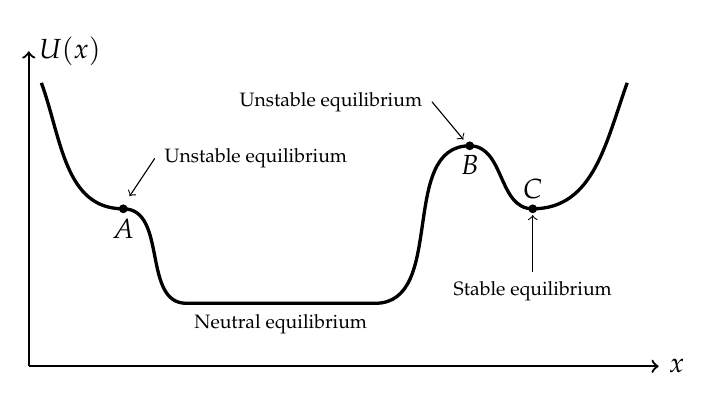
\begin{tikzpicture}[scale=.8]
      \draw[thick,->](0,0)--(10,0) node[right]{$x$};
      \draw[thick,->](0,0)--(0,5) node[right]{$U(x)$};
      \draw[very thick](.2,4.5) to[out=-70,in=180](1.5,2.5)
      to[out=0,in=180](2.5,1)
      --(5.5,1) node[midway,below]{\scriptsize Neutral equilibrium}
      to[out=0,in=180](7,3.5)
      to[out=0,in=180](8,2.5)
      to[out=0,in=250](9.5,4.5);
      \fill(1.5,2.5) circle(.07) node[below]{$A$};
      \fill(7,3.5)   circle(.07) node[below]{$B$};
      \fill(8,2.5)   circle(.07) node[above]{$C$};
      \draw[<-](1.6,2.7)--(2,3.3) node[right]{\scriptsize Unstable equilibrium};
      \draw[<-](6.9,3.6)--(6.4,4.2)node[left]{\scriptsize Unstable equilibrium};
      \draw[<-](8,2.4)--(8,1.5)node[below]{\scriptsize Stable equilibrium};
    \end{tikzpicture}
  \end{center}
\end{frame}


\section{Power \& Efficiency}

\begin{frame}{Power}
  \textbf{Power} is the \emph{rate} at which work is done, i.e.\ the rate at
  which energy is being transformed:

  \eq{-.2in}{
    \boxed{P(t) = \diff Wt}\quad\quad
    \boxed{\overline P = \frac W{\Delta t}}
  }
  \begin{center}
    \begin{tabular}{l|c|c}
      \rowcolor{pink}
      \textbf{Quantity}  & \textbf{Symbol} & \textbf{SI Unit} \\ \hline
      Instantaneous and average power & $P$, $\overline P$ & \si\watt \\
      Work done          & $W$ & \si\joule \\
      Time interval      & $\Delta t$ & \si\second
    \end{tabular}
  \end{center}
  In engineering, power is often more critical than the actual amount of work
  done.
\end{frame}



\begin{frame}{Power}
  If a constant force is used to push an object at a constant velocity, the
  power produced by the force is:
  
  \eq{-.1in}{
    P=\diff Wt=\frac{\bm F\cdot\dl\bm x}{\dl t}
    =\bm F\cdot\diff{\bm x}t
    \quad\rightarrow\quad
    \boxed{P=\bm F\cdot\bm v}
  }
  
  Application: aerodynamics
  \begin{itemize}
  \item When an object moves through air, the applied force must overcome air
    resistance (drag force), which is proportional with $v^2$
    \item Therefore ``aerodynamic power'' must scale with $v^3$ (i.e.\ doubling
      your speed requires $2^3=8$ times more power)
    \item Important when aerodynamic forces dominate
  \end{itemize}
\end{frame}



\begin{frame}{Efficiency}
  \textbf{Efficiency} is the ratio of useful energy or work output to the total
  energy or work input

  \eq{-.2in}{
    \boxed{ \eta = \frac{E_o}{E_i}\times\SI{100}\percent }\quad
    \boxed{ \eta = \frac{W_o}{W_i}\times\SI{100}\percent }
  }
  \begin{center}
    \begin{tabular}{l|c|c}
      \rowcolor{pink}
      \textbf{Quantity} & \textbf{Symbol} & \textbf{SI Unit} \\ \hline
      Useful output energy & $E_o$  & \si\joule \\
      Input energy         & $E_i$  & \si\joule \\
      Useful output work   & $W_o$  & \si\joule \\
      Input work           & $W_i$  & \si\joule \\
      Efficiency           & $\eta$ & no units
    \end{tabular}
  \end{center}
  Efficiency is always $0\leq\eta<\SI{100}\percent$
\end{frame}
\end{document}
